\documentclass[a4paper]{article}
\usepackage{geometry}
\usepackage{fontawesome}
\usepackage{titlesec}
\usepackage{enumitem}
\usepackage{xcolor}
\usepackage{hyperref}
\usepackage{graphicx}

% Page settings
\geometry{left=1.8cm,right=1.8cm,top=1cm,bottom=1cm,includefoot}

% Color definitions
\definecolor{mainred}{RGB}{204,0,0}
\definecolor{darkgray}{RGB}{73,73,73}

% Hyperlink settings
\hypersetup{
    colorlinks=true,
    linkcolor=mainred,
    filecolor=mainred,
    urlcolor=darkgray,
}

% Section title format
\titleformat{\section}
{\color{mainred}\Large\bfseries}
{}{0em}{\faGraduationCap\quad}[\titlerule]
\titlespacing{\section}{0pt}{10pt}{6pt}

% Line spacing
\linespread{1.1}

\begin{document}
% remove page number
\pagenumbering{gobble}

% Header
\begin{minipage}{0.75\textwidth}
\hspace{-1em}
{\huge\bfseries Qiwei Chen}\medskip

\vspace{0.5em}
\hspace{-0.5em}
\begin{tabular}{@{}l@{\hspace{0.4em}}l@{\hspace{3.5em}}l@{}}
{\color{darkgray}\faPhone} & +86 131-2312-8852 & {\color{darkgray}\faCalendar} Sep 21, 2003 \\
{\color{darkgray}\faEnvelope} & qiweic10@sjtu.edu.cn & {\color{darkgray}\faUser} CPC Probationary Member \\
{\color{darkgray}\faGithub} & \href{https://github.com/kiwi142857}{\color{darkgray}kiwi142857} & {\color{darkgray}\faHome} \href{https://kiwi142857.github.io/kiwi142857.githhub.io/}{\color{darkgray}Portfolio}
\end{tabular}
\end{minipage}
\begin{minipage}{0.25\textwidth}
\hspace{0.5em}
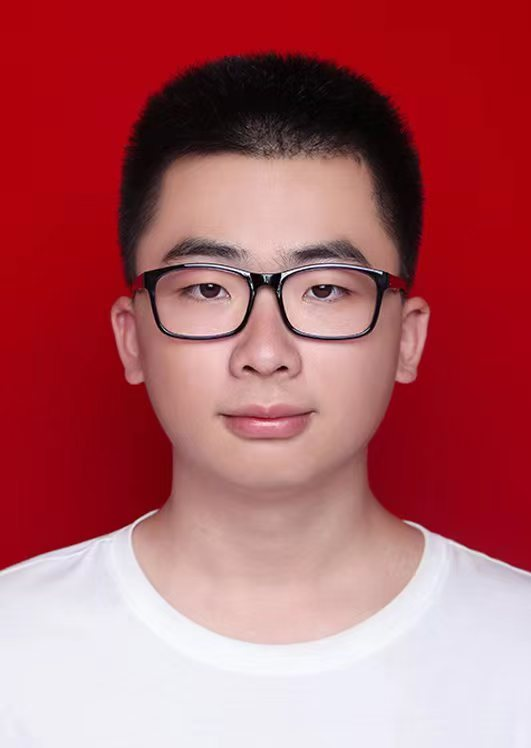
\includegraphics[width=2.8cm]{Kiwi_陈启炜.jpg}
\end{minipage}

\vspace{-2.2em}
\section*{Education}
\noindent\textbf{\large Shanghai Jiao Tong University} \textbf{Software Engineering} \hfill Sep 2022 - Present\\
\vspace{1em}
\textit{Academic Score: 91.0/100 (Rank: 7/93)} \hfill \textit{GPA: 3.91/4.30 (Rank: 12/93)}\\

\vspace{-1.8em}
\noindent\textbf{Honors}
\begin{itemize}[leftmargin=*,itemsep=0em,topsep=0em]
\item Jiang Scholarship \hfill 2023-2024
\item Outstanding Undergraduate Scholarship, SJTU \hfill 2022-2024
\item Outstanding Student Leader \& League Member, SJTU \hfill 2023-2024
\end{itemize}

\section*{Projects}
\begin{itemize}[leftmargin=*,label={},itemsep=0.3em,topsep=0.1em]
\item \textbf{\href{https://gitee.com/qiweic10/open-trustee_-llm_app}{OpenTrustee LLM}} \hfill \textit{2024.09 - 2024.11}\\
Led the development of secure LLM inference deployment on edge devices using OpenTrustee and llama.cpp. Designed and implemented model loading and inference modules in TEE environment, ensuring model parameter security through hardware encryption. Won Third Prize in OpenHarmony National Competition.

\item \textbf{Tiger Language Compiler} \hfill \textit{2024.09 - 2025.01}\\
Designed and implemented a Tiger compiler with Flex/Bison for lexical/syntax analysis and AST for semantic analysis. Optimized code generation via stack frame management and register allocation. Enhanced performance through LLVM-based multi-level optimization.

\item \textbf{\href{https://github.com/kiwi142857/CSE-chfs}{CHFS Distributed File System}} \hfill \textit{2024.09 - 2025.01}\\
Designed and implemented a GFS-based distributed file system. Managed file metadata using Inode mechanism, implemented logging and snapshot features for data reliability. Achieved multi-replica consistency using Raft algorithm with automatic failure recovery. Supported concurrent requests and large-scale file storage with fast retrieval capabilities.

\item \textbf{\href{https://github.com/UniGPT-SJTU}{UniGPT Prompt Platform}} \hfill \textit{2024.02 - 2024.09}\\
Led a 4-person team in agile development. Designed microservices architecture and implemented k8s-based deployment pipeline. Integrated LLM capabilities with langchain4j for intelligent prompt recommendations. Won Excellence Award in Software Exhibition.

\item \textbf{\href{https://github.com/kiwi142857/LSM-Tree}{LSM-Tree Key-Value Store}} \hfill \textit{2024.04 - 2024.06}\\
Independently implemented an LSM-Tree based key-value storage system. Developed skiplist index structure in C++ supporting efficient insertion, deletion, and query operations. Ensured data persistence through WAL mechanism, optimized read performance using LSM-Tree, and reduced read amplification with Bloom filters.

\section*{Leadership \& Activities \& Internship}
\hspace{-0.5cm}
\begin{minipage}[t]{0.38\textwidth}
\textbf{Student Leadership}
\begin{itemize}[leftmargin=*,itemsep=0em,topsep=0em]
\item Student Union Member, SEIEE
\item Class Committee Member
\item Member of "Si Yuan" Program
\end{itemize}
\end{minipage}
\begin{minipage}[t]{0.38\textwidth}
\textbf{Social Practice}
\begin{itemize}[leftmargin=*,itemsep=0.1em,topsep=0.1em]
\item Social Research Project in Hunan
\item Greater Bay Area Investigation
\end{itemize}
\end{minipage}
\begin{minipage}[t]{0.24\textwidth}
\textbf{Internship}
\begin{itemize}[leftmargin=*,itemsep=0.1em,topsep=0.1em]
\item Jiangran Technology\\
\textit{2025.01 - 2025.02}
\end{itemize}
\end{minipage}
\section*{Technical Skills}
\begin{itemize}[leftmargin=*,itemsep=0.1em,topsep=0.1em]
\item \textbf{Programming Languages}: Proficient in C/C++; Skilled in Python, Java, JavaScript; Familiar with Swift
\item \textbf{Development Skills}: Microservices Architecture, DevOps, LLM Deployment, Secure Computing, Distributed Systems, llama.cpp
\item \textbf{Language Skills}: CET-6 Certification, Strong Technical Documentation Abilities
\end{itemize}

\end{document} 